\documentclass[conference]{IEEEtran}
% for subfigure 
\usepackage{caption}
\usepackage{subcaption}
% to have reference and index in table of content
\usepackage{tocbibind}
% to have index
\usepackage{makeidx}
\makeindex

\usepackage{graphicx}
%\graphicspath{{figures/}}
\usepackage{amsmath}

\usepackage{hyperref}

% for tabels
\usepackage{multirow}
\usepackage[table,xcdraw]{xcolor}
% for khafan enumrate
\usepackage[inline]{enumitem}
%%%%%%%%%%%%%%%%%%%%%%%%%%
% xepersian and fonts
\usepackage{xepersian}
\settextfont{XBZar}
\setdigitfont{XBZar}
%%%%%%%%%%%%%
\defpersianfont\titr[Scale=1]{XB Zar}
\defpersianfont\nastaliq[Scale=1.5]{IranNastaliq}
\defpersianfont\traffic[Scale=1]{XM Traffic}
%%%%%%%%%%%%%%%%%%%%%%%%%%
\begin{document}

\title{Comparing Some Case Of Density-based Spatial Clustering Of Applications With Noise (DBSCAN) With Changing Data And Algorithm Parameter(HW3) \\
	{\footnotesize \textsuperscript{}
	}
	\thanks{}
}

\author{\IEEEauthorblockN{AmirHossein Asadi}
	\IEEEauthorblockA{\textit{Computer Engineering Department} \\
		\textit{Shahid Rajaee Teacher Training University}\\
		Tehran, Iran \\
		amirasadi@sru.ac.ir}}


\maketitle
\begin{abstract}
In this homework first we review the concepts of clustering specially density based ones and equations and concept behind them. then we show the results of DBSCAN in six different condition. after that discuss about the results.
\end{abstract}

\begin{IEEEkeywords}
	 Clustering, Density Based Clustering, DBSCAN, Clustering Evaluation
\end{IEEEkeywords}


\section{Introduction}
``Cluster analysis or clustering is the task of grouping a set of objects in such a way that objects in the same group (called a cluster) are more similar (in some sense) to each other than to those in other groups (clusters)''\cite{enwiki:1005655155}
\newline
% why clustering
We use clustering when have some data with out label or tag for example consider we have a lot of height and weight measurements of cat and dog and wants to group them without knowing the animal type. these groups of algorithm called unsupervised learning in machine learning. in reality there are more situations that you have the data but you don't have the label.
\newline
These algorithms have many application such as: bioinformatics, Medicine, Business and marketing, World wide web, Computer science, Social science and etc. for example in medical imaging clustering can help to differentiate between different types of tissue in a three-dimensional image for many different purposes\cite{filipovych2011semi}.
There are many way you can separate clustering methods one of them depends on nature of algorithms.
In thins manner wen can define five different type of clustering algorithms including:
\begin{enumerate}
	\item Connectivity-based clustering (hierarchical clustering)
	\item Centroid-based clustering
	\item Distribution-based clustering
	\item Density-based clustering
	\item Grid-based clustering
\end{enumerate}
In this homework we want to analyses some cases with different data and parameters of Density-based Spatial Clustering Of Applications With Noise - DBSCAN method. as the algorithm name shows this algorithm belongs to forth group, named Density-based clustering.
\newline
In density based approaches we define a group of data a cluster if they have enough density and objects in spare areas are considered noise or border points.DBSCAN and OPTICS\footnote{Ordering points to identify the clustering structure} are most known in density based approaches. we can say OPTICS is generalized form of DBSCAN.
\newline
It was first introduced in 1996 by Ester et al \cite{ester1996density}.
The advantages of this algorithm against other approaches are that in this method data could be in any shape and form while in k-means data must be compact and not in complex forms. another benefit is that there is no need to define value of k the algorithm observe all the data and add cluster if it is needed.
\section{Methods}
DBSCAN has two main parameters epsiolon($\epsilon$) and minPoint.
$\epsilon$ defines the distance to search for object and minPoint defines minimum number of objects to be dense. there are three type of point in DBSCAN:
\begin{itemize}
	\item Core
	\item Border
	\item Noise
\end{itemize}
Core is a point which has at least p point in distance d. Border is a point that has at lease one core point at distance d, and Noise is a point that there is less than p point in distance d or in other word it is not core nor border.
\textbf{Reachability} means if a point distance is less than $\epsilon$ it is reachable.
\textbf{Connectivity} means when two points are connected through reachable dense space. you can see an example in figure \ref{fig:dbscan-example}.
\begin{figure}[h]
	\centering
	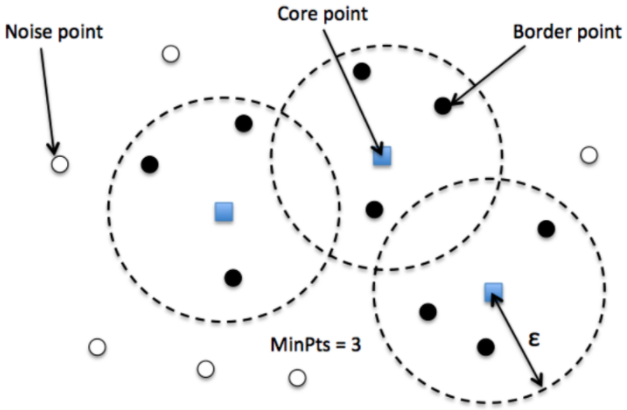
\includegraphics[width=0.9\linewidth]{figures/DBSCAN-example}
	\caption{Example of DBSCAN and its definitions\cite{kdnuggetsDBSCAN}.}
	\label{fig:dbscan-example}
\end{figure}
the method can be summery in algorithm \ref{alg:alg1}.

\begin{algorithm}
	\KwIn{$\epsilon$, MinPoint, DistanceFunction, DB}
	set $ X_{un} = X$ \\
	set $ m = 0 $ \tcp*{Cluster counter}
	\While{$ X_{un} \neq \O$}{
		Arbitrarily select a $ x \in X_{un}$ \\
		\If{$ x $ \text{is a noncore point}}{
			Mark $ x $ as a noise point\\
			$ X_{un} = X_{un} - \{x\} $\\
		}
		\If{$ x $ is a core point}{
			$ m = m + 1 $\\
			Determine all density-reachable points in $ X $ from $ x $\\
			Assign $ x $ and the previous points to the cluster $ C_m $\\
			The border points that may have been marked as noise are also assigned to $ C_m $\\
			$ X_{un} = X_{un} - C_m $\\
		}
	}
	\caption{DBSCAN pseudocode}
	\label{alg:alg1}
\end{algorithm}
\section{Results}
\label{sec:result}
In this section we run six different case for DBSCAN algorithm some changes in input data and other in algorithm it self.all codes and implementation are done with python 3.8.5 and sklearn package\cite{scikit-learn}. you can see the experiments and their details in table \ref{tab:experiments}.
\begin{table}
	\centering
	\caption{Summery of designed experiments}
	\label{tab:experiments}
	\begin{tabular}{ll}\toprule
		\textbf{Experiment NO} & \textbf{Details}\\
		\midrule
		base & Bolbs dataset, $\epsilon$ = 3, MinPoint = 3\\ \midrule\midrule
		1 & No Structure \\
		2 & Noisy Moon dataset \\
		3 & Noisy Circles dataset \\ \midrule 
		4 &  Manhattan distance \\ 
		5 &  $ \epsilon = 0.5 $ \\
		6 &  MinPoint = 5 \\ \bottomrule
	\end{tabular}
\end{table}
We can see the result of clustering for base condition in figure \ref{fig:bolb} and its confusion matrix in figure \ref{fig:cmbolb}. the first row of confusion matrix is for noise data.
and then we run the algorithm in cases that we just change the input data but with the same algorithm parameter in base condition. the result is show in figure \ref{fig:panel1}.
\begin{figure}[h]
	\centering
	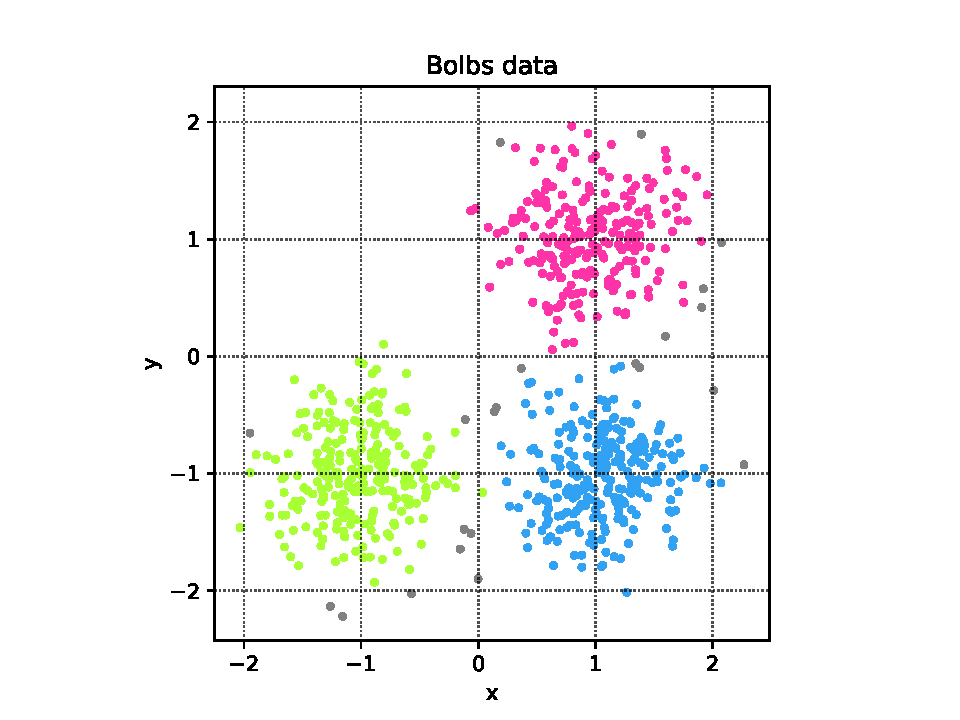
\includegraphics[width=1\linewidth]{figures/bolb}
	\caption{DBSCAN in base experiment, gray points are considered as noise}
	\label{fig:bolb}
\end{figure}
\begin{figure}[h]
	\centering
	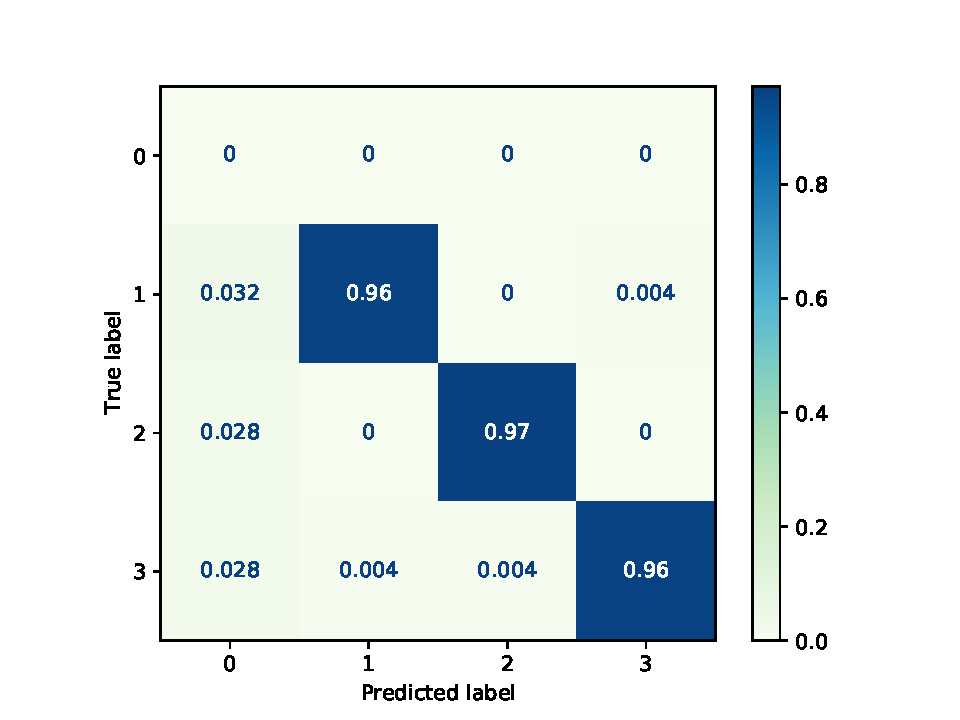
\includegraphics[width=1\linewidth]{figures/cm_bolb}
	\caption{Normalized confusion matrix}
	\label{fig:cmbolb}
\end{figure}

\begin{figure*}[h]
	\begin{subfigure}{0.33\linewidth}
		\centering
		% include first image
		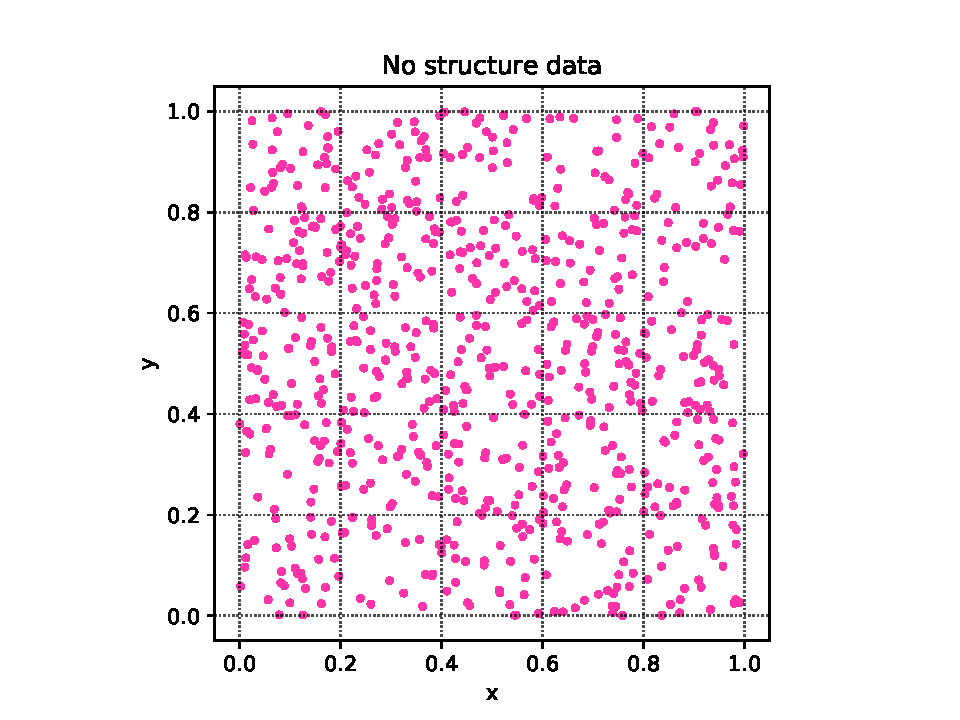
\includegraphics[width=\linewidth]{figures/1-NoStructure}  
		\caption{DBSCAN in first experiment}
		\label{fig:p1-1}
	\end{subfigure}
	\begin{subfigure}{0.33\textwidth}
		\centering
		% include image 2
		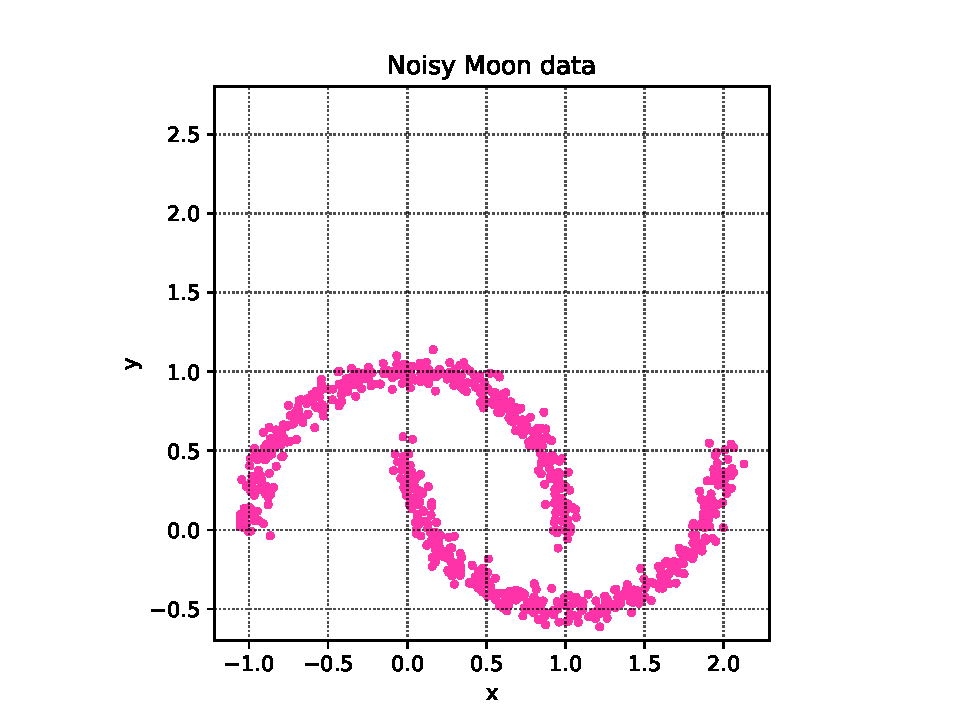
\includegraphics[width=\linewidth]{figures/2-NoisyMoon}
		\caption{DBSCAN in second experiment}
		\label{fig:p1-2}
	\end{subfigure}
	\begin{subfigure}{0.33\textwidth}
		\centering
		% include image 3
		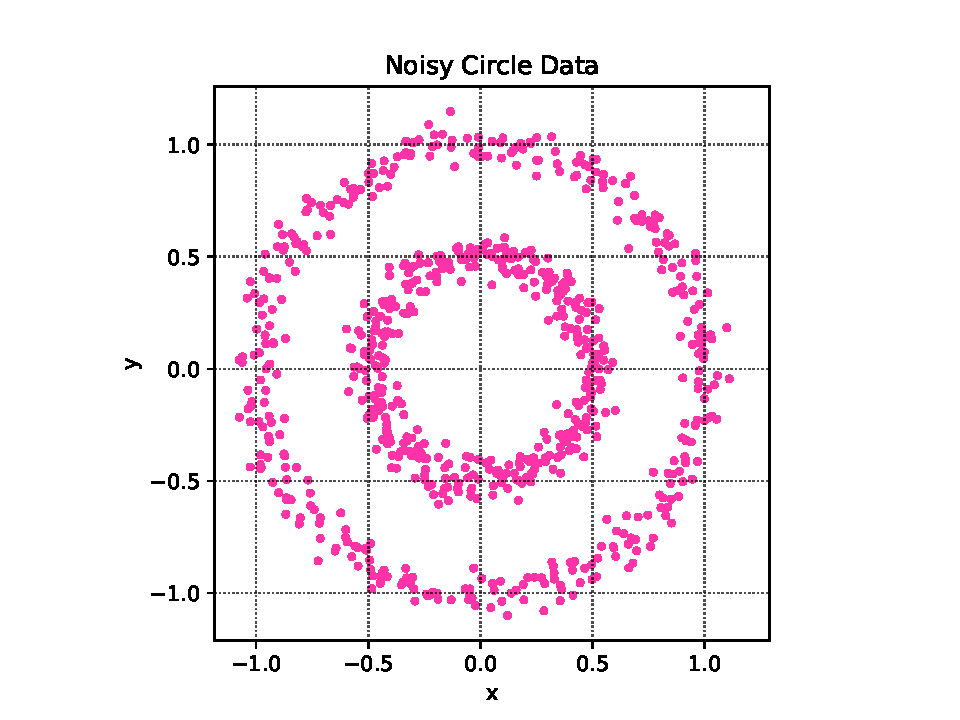
\includegraphics[width=\linewidth]{figures/3-NoisyCircle}
		\caption{DBSCAN in third experiment}
		\label{fig:p1-3}
	\end{subfigure}	
	
	
	\begin{subfigure}{0.33\textwidth}
		\centering
		% include image 4
		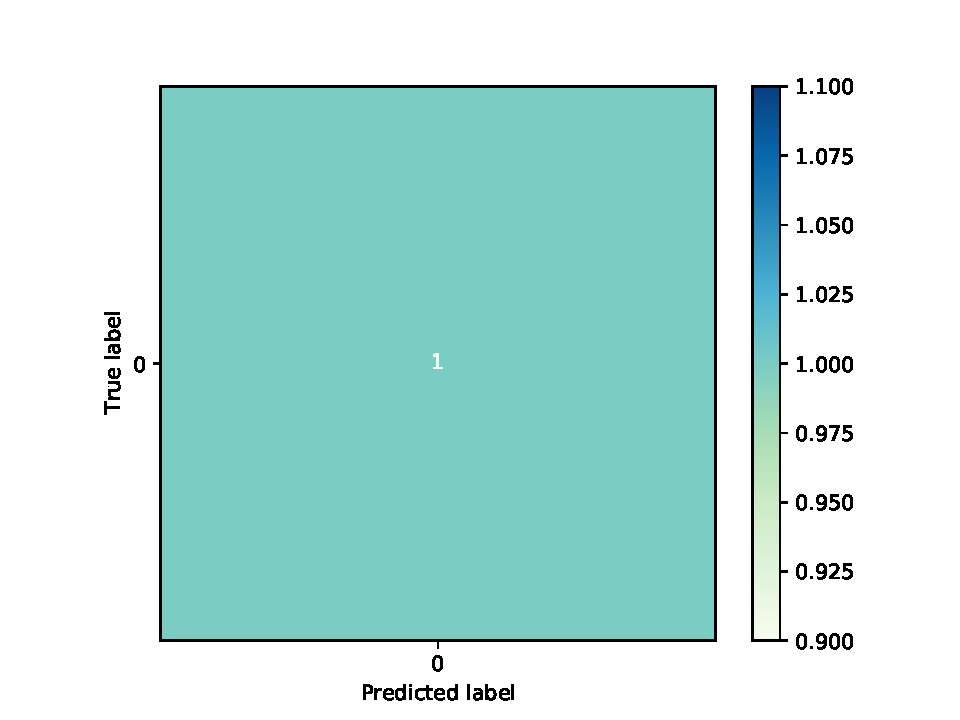
\includegraphics[width=\linewidth]{figures/1-cm-NoStructure}
		\caption{Confusion matrix of no structure data}
		\label{fig:p1-4}
	\end{subfigure}
	\begin{subfigure}{0.33\textwidth}
		\centering
		% include image 5
		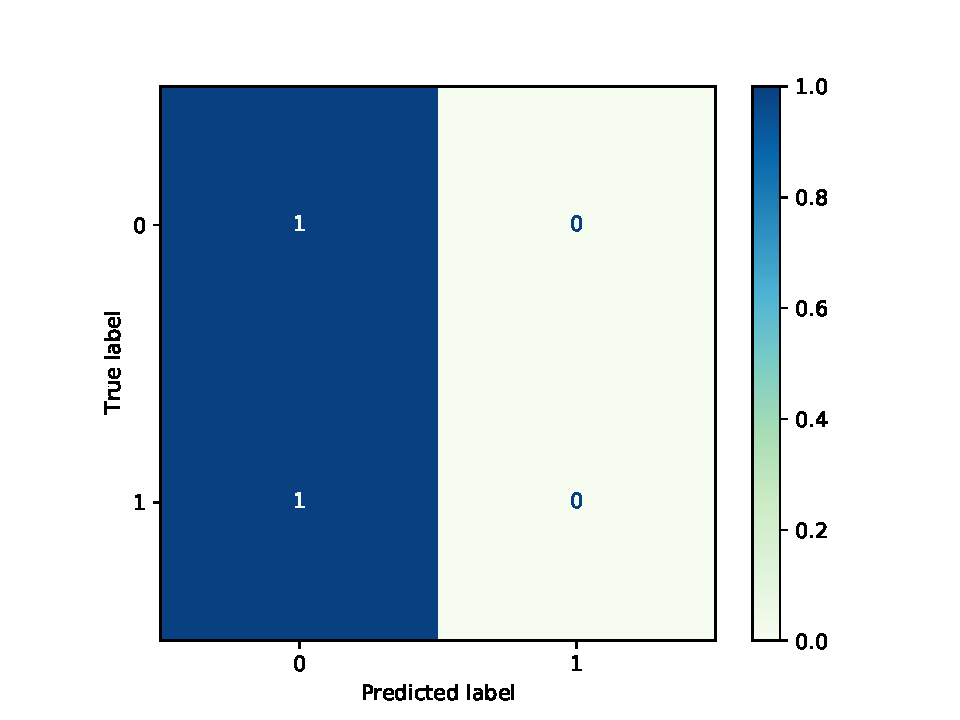
\includegraphics[width=\linewidth]{figures/2-cm-NoisyMoon}  
		\caption{Confusion matrix of noisy moon data}
		\label{fig:p1-5}
	\end{subfigure}
	\begin{subfigure}{0.33\textwidth}
		\centering
		% include image 6
		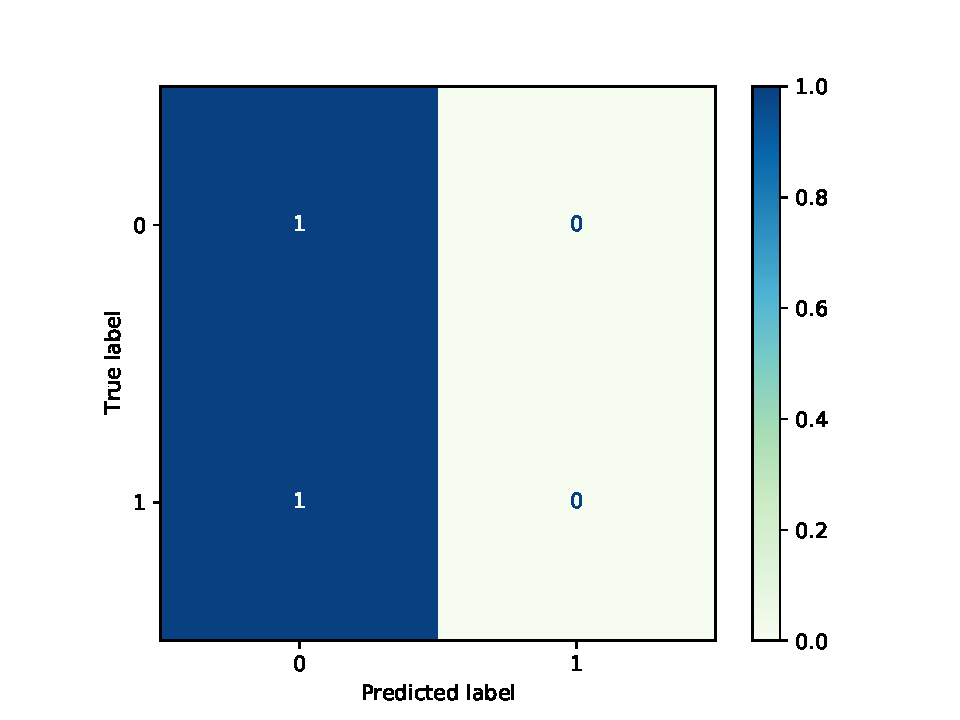
\includegraphics[width=\linewidth]{figures/3-cm-NoisyCircle}  
		\caption{Confusion matrix of noisy circle data}
		\label{fig:p1-6}
	\end{subfigure}
	\caption{Result of first \subref{fig:p1-1} three experiment as you can see in \cref{fig:p1-1,fig:p1-2} DBSCAN just found one cluster while there is two, and this is because of setting its parameters not precise.}
	\label{fig:panel1}
\end{figure*}
In figure \ref{fig:panel2} you can see the results when we change the parameters of algorithm such as metric function, $\epsilon$ and MinPoint.
\begin{figure*}[h]
	\begin{subfigure}{0.33\textwidth}
		\centering
		% include first image
		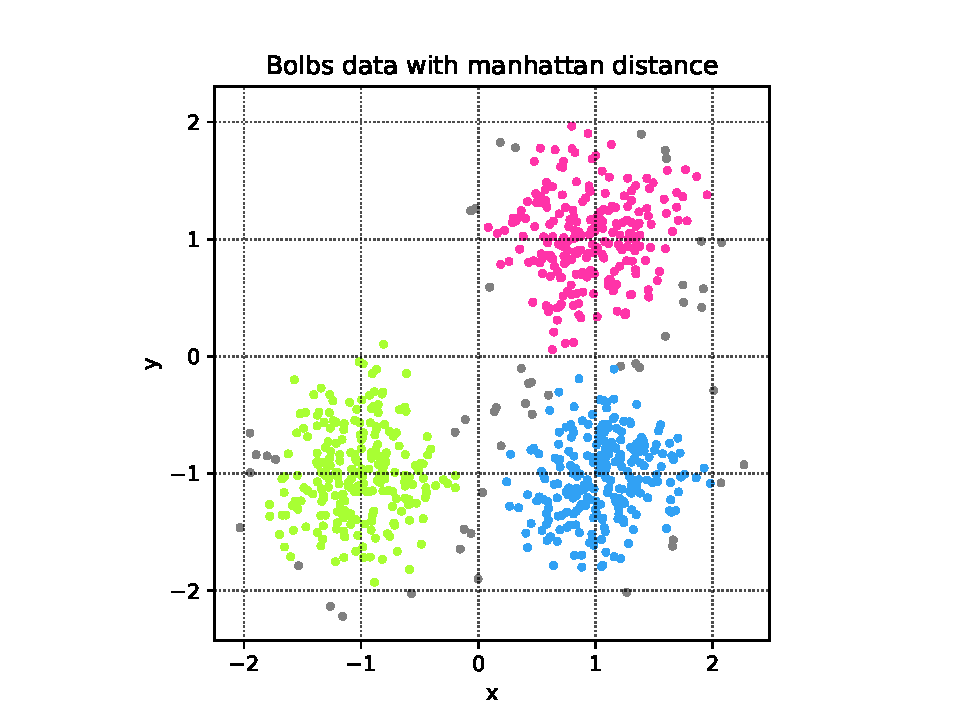
\includegraphics[width=\linewidth]{figures/4-bolb}  
		\caption{DBSCAN result in forth experiment}
		\label{fig:p2-1}
	\end{subfigure}
	\begin{subfigure}{0.33\textwidth}
		\centering
		% include image 2
		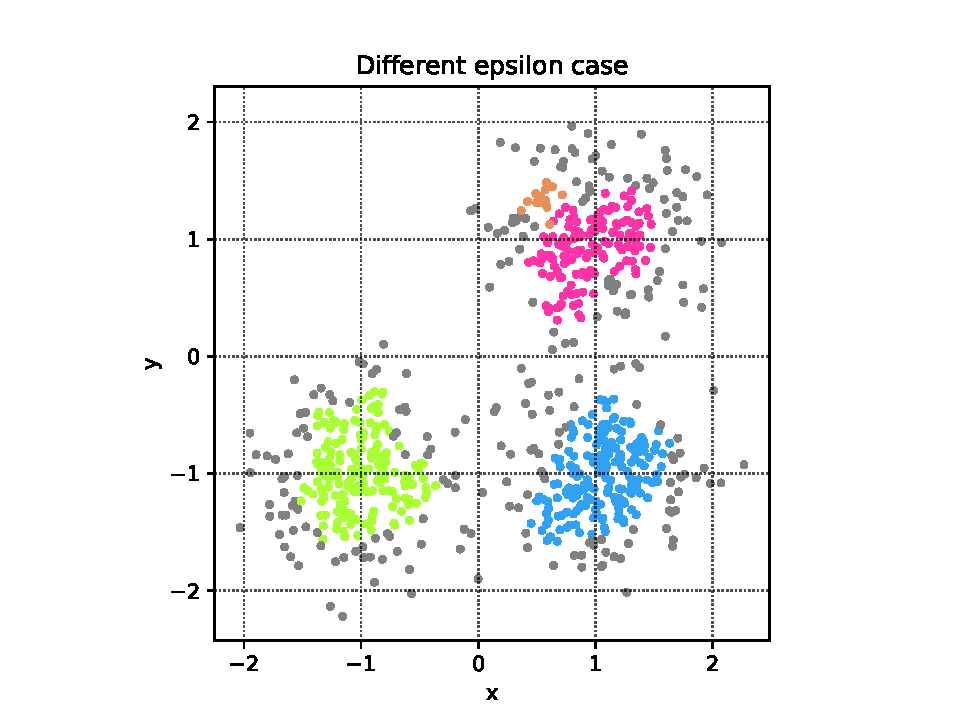
\includegraphics[width=\linewidth]{figures/5-epsilon}
		\caption{DBSCAN result in fifth experiment}
		\label{fig:p2-2}
	\end{subfigure}
	\begin{subfigure}{0.33\textwidth}
		\centering
		% include image 3
		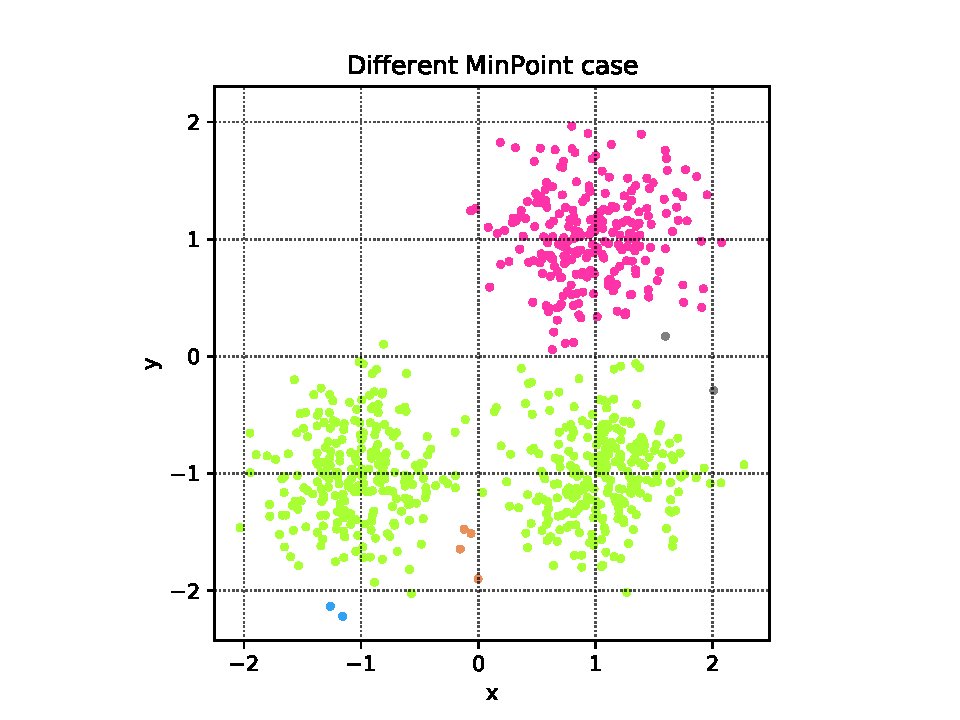
\includegraphics[width=\linewidth]{figures/6-MinPoint}
		\caption{DBSCAN result in sixth experiment}
		\label{fig:p2-3}
	\end{subfigure}	
	
	
	\begin{subfigure}{0.33\textwidth}
		\centering
		% include image 4
		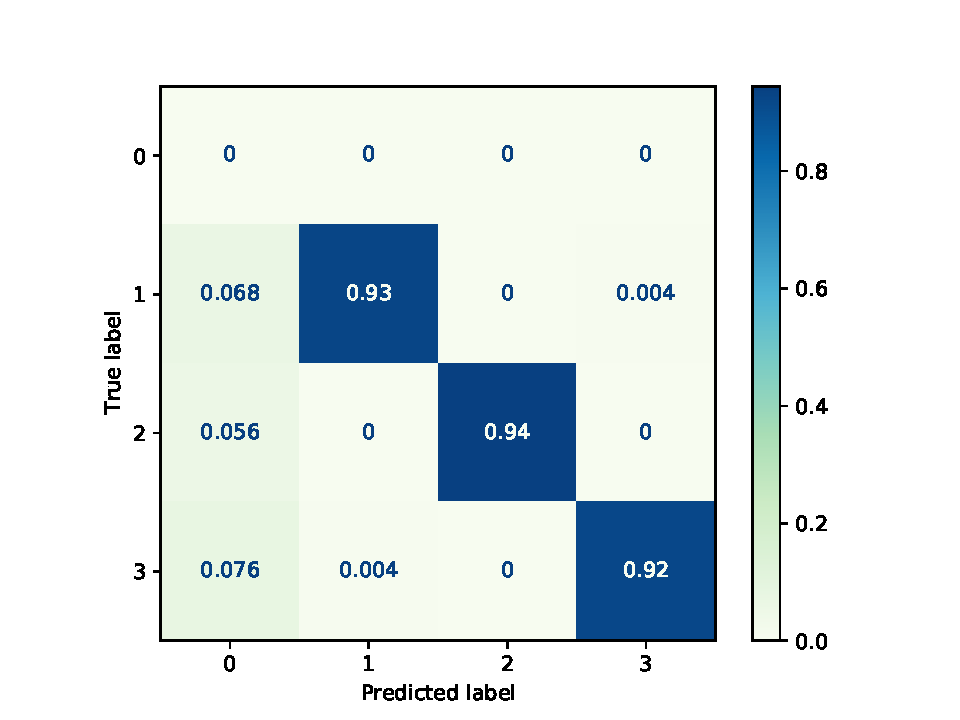
\includegraphics[width=\linewidth]{figures/4-cm_bolb}
		\caption{Confusion matrix of manhattan distance}
		\label{fig:p2-4}
	\end{subfigure}
	\begin{subfigure}{0.33\textwidth}
		\centering
		% include image 5
		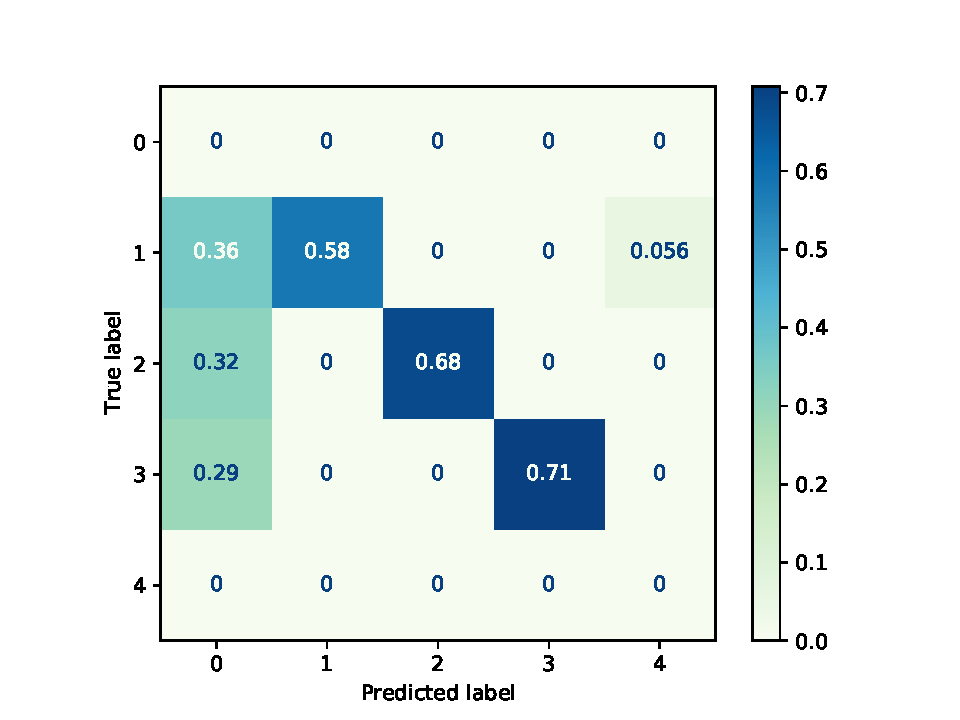
\includegraphics[width=\linewidth]{figures/5-cm-epsilon}  
		\caption{Confusion matrix of $\epsilon = 0.15$  }
		\label{fig:p2-5}
	\end{subfigure}
	\begin{subfigure}{0.33\textwidth}
		\centering
		% include image 6
		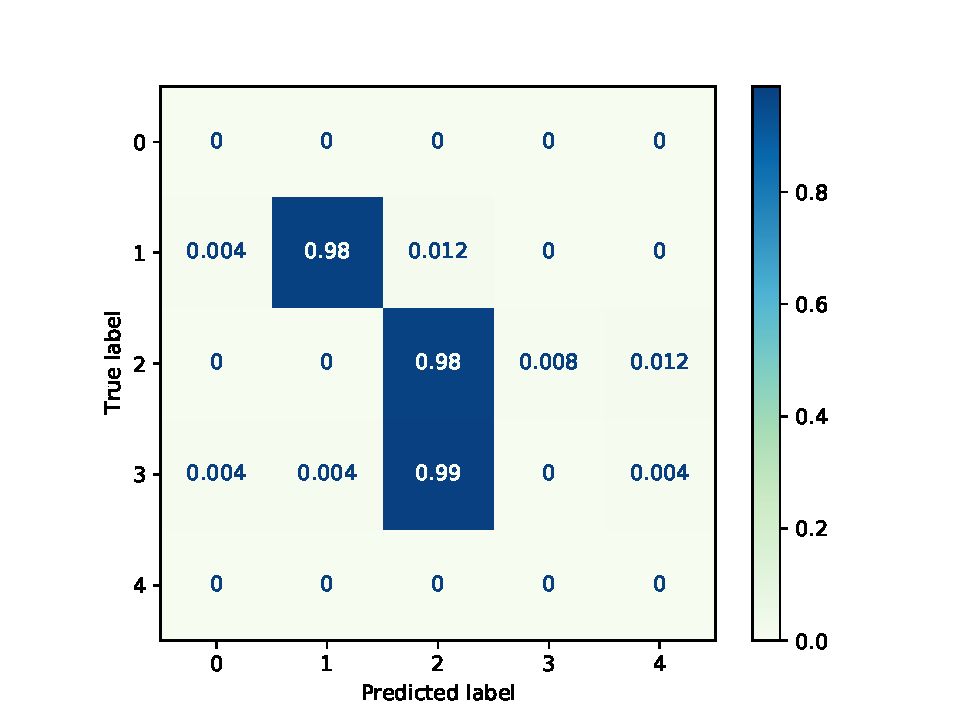
\includegraphics[width=\linewidth]{figures/6-cm-MinPoint}  
		\caption{Confusion matrix of MinPoint = 2 }
		\label{fig:p2-6}
	\end{subfigure}
	\caption{Result of second three experiment, here we change parameters of DBSCAN such as metric function, $\epsilon$ and MinPoint.}
	\label{fig:panel2}
\end{figure*}

in table \cref{tab:1,tab:2,tab:3,tab:4,tab:5,tab:6,tab:base} you can see the result of evaluating the clustering methods.
\begin{table}[]
	\centering
	\caption{Evaluation of base case accuracy was 0.97}
	\label{tab:base}
	\begin{tabular}{cccc}
		\textbf{Label} & \textbf{precision} & \textbf{recall} & \textbf{f1-score} \\
		\hline
		0 & 1.00 & 0.96 & 0.98 \\
		1 & 1.00 & 0.97 & 0.98 \\
		2 & 1.00 & 0.96 & 0.98
	\end{tabular}
\end{table}

\begin{table}[]
	\centering
	\caption{Evaluation of first case accuracy was 1.00}
	\label{tab:1}
	\begin{tabular}{cccc}
		\textbf{Label} & \textbf{precision} & \textbf{recall} & \textbf{f1-score} \\
		\hline
		0 & 1.00 & 1.00 & 1.00 
	\end{tabular}
\end{table}

\begin{table}[]
	\centering
	\caption{Evaluation of second case accuracy was 0.50}
	\label{tab:2}
	\begin{tabular}{cccc}
		\textbf{Label} & \textbf{precision} & \textbf{recall} & \textbf{f1-score} \\
		\hline
		0 & 0.50 & 1.00 & 0.67\\
		1 & 0.00 & 0.00 & 0.00
	\end{tabular}
\end{table}

\begin{table}[]
	\centering
	\caption{Evaluation of third case accuracy was 0.50}
	\label{tab:3}
	\begin{tabular}{cccc}
		\textbf{Label} & \textbf{precision} & \textbf{recall} & \textbf{f1-score} \\
		\hline
		0       &0.50 &     1.00  &    0.67 \\
		1       &0.00&      0.00   &   0.00 
	\end{tabular}
\end{table}

\begin{table}[]
	\centering
	\caption{Evaluation of forth case accuracy was 0.93}
	\label{tab:4}
	\begin{tabular}{cccc}
		\textbf{Label} & \textbf{precision} & \textbf{recall} & \textbf{f1-score} \\
		\hline
		  -1    &   0.00  &    0.00   &   0.00  \\       
			0    &   1.00  &    0.93   &   0.96  \\
			1    &   1.00  &    0.94   &   0.97  \\
			2    &  1.00   &    0.92   & 0.96    \\
	\end{tabular}
\end{table}

\begin{table}[]
	\centering
	\caption{Evaluation of fifth case accuracy was 0.66}
	\label{tab:5}
	\begin{tabular}{cccc}
		\textbf{Label} & \textbf{precision} & \textbf{recall} & \textbf{f1-score} \\
		\hline
          -1   &   0.00  &    0.00  &    0.00     \\
			0   &   1.00  &    0.98  &    0.99     \\
			1   &   0.49  &    0.98  &    0.66     \\
			2   &   0.00  &    0.00  &    0.00     \\
			3   &   0.00  &    0.00  &    0.00     \\
	\end{tabular}
\end{table}

\begin{table}[]
	\centering
	\caption{Evaluation of sixth case accuracy was 0.65}
	\label{tab:6}
	\begin{tabular}{cccc}
		\textbf{Label} & \textbf{precision} & \textbf{recall} & \textbf{f1-score} \\
		\hline
          -1    &   0.00   &   0.00    &  0.00     \\
			0    &   1.00   &   0.98    &  0.99     \\
			1    &   0.49   &   0.98    &  0.66     \\
			2    &   0.00   &   0.00    &  0.00     \\
			3    &   0.00   &   0.00    &  0.00     \\
	\end{tabular}
\end{table}


\begin{figure}[h]
	\centering
	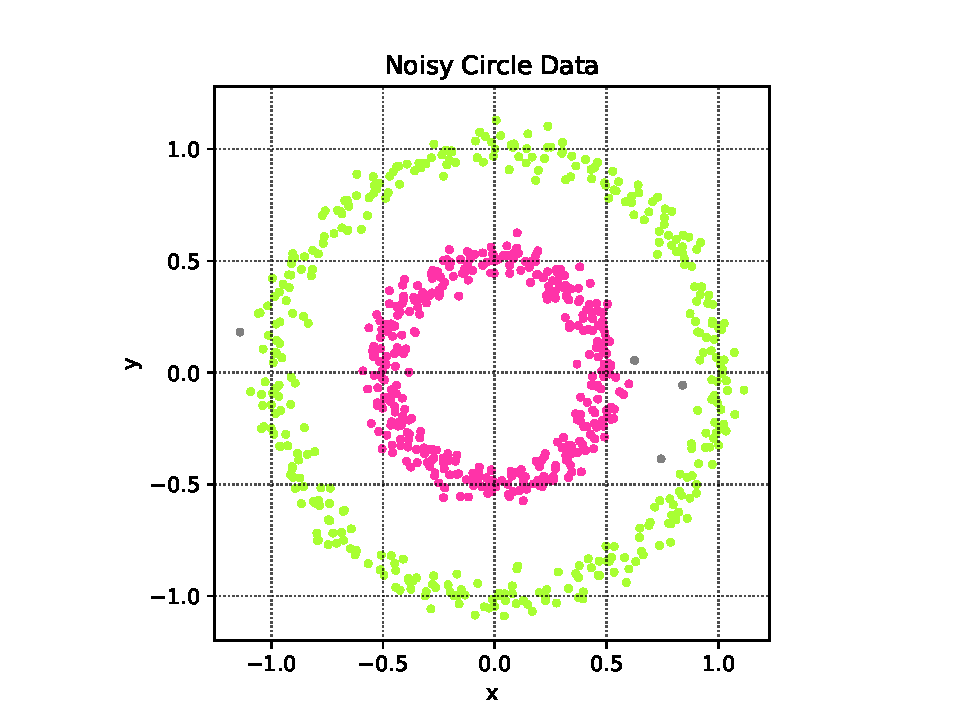
\includegraphics[width=1\linewidth]{figures/NoisyCircleTune}
	\caption{Noisy Cricle with $\epsilon = 0.1$ and MinPoint=3}
	\label{fig:noisycircletune}
\end{figure}

\begin{figure}[h]
	\centering
	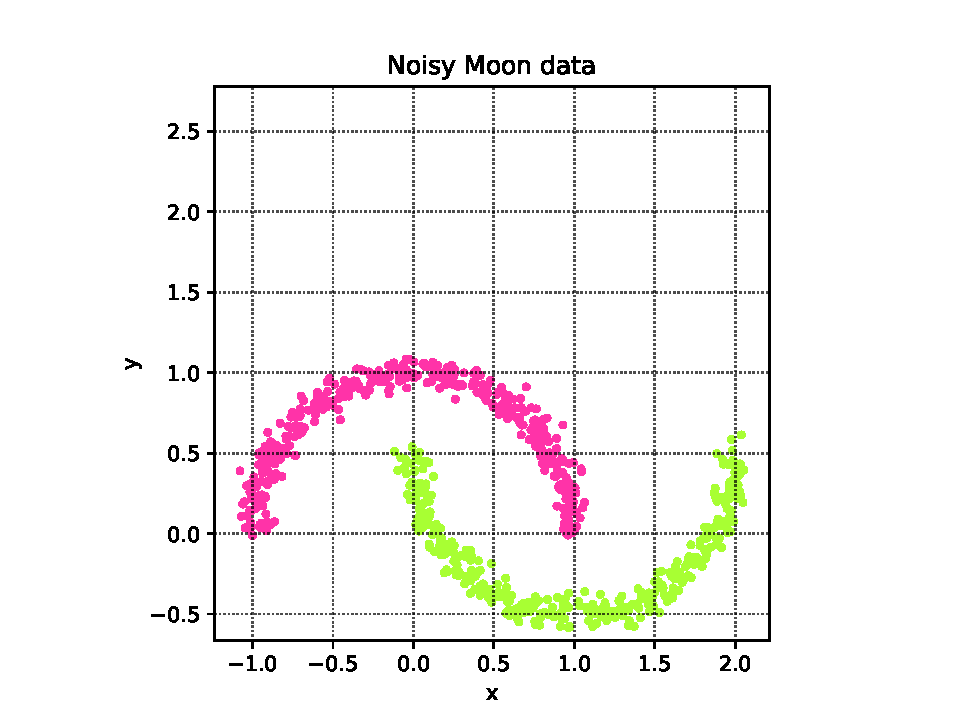
\includegraphics[width=1\linewidth]{figures/NoisyMoonTune}
	\caption{Noisy Moon with  $\epsilon = 0.3$ and MinPoint = 10}
	\label{fig:noisymoontune}
\end{figure}

\section{Discussion}
In section \ref{sec:result} we see the results of our clustering in base and six different case and after that their evaluation with five different measure including: precision, recall, f1-score and confusion matrix.
\\
From the results we understand DBSCAN has three main parameter
\begin{enumerate}
	\item $ \epsilon $
	\item MinPoint
	\item Distance Function
\end{enumerate}
These six experiment show if we make $\epsilon$ smaller it will make more data as noise and on the other side if we choose larger value we have less noise data but if it is large enough it may merge two cluster.
\newline
The other parameter is MinPoint results shows that if we choose smaller value it will make more clusters which maybe they are not actually cluster figure \ref{fig:p2-3} is example of that on the other hand if we choose large value for MinPoint as it requires lots of point to be dense then we may have more border points and noise point.
\\
Testing many different distance function such as: cityblock, cosine, euclidean, l1, l2, manhattan’ ‘braycurtis, canberra, chebyshev, correlation, dice, hamming, jaccard, kulsinski, mahalanobis, minkowski, rogerstanimoto, russellrao, seuclidean, sokalmichener, sokalsneath, sqeuclidean and yule show that the default one(euclidean) has the best results and after that manhattan distance while most of others function fails badly and could find just one cluster in three circle cluster.
\section{Conclusion}
In this homework we use synthesis some data to analyses DBSCAN algorithm with different parameters and to measure the quality of our results we use five different evaluation measurement. we design six different case which three of them has different input data and others has different algorithm parameters and one base case to compare them.
\newline
Results shows that if parameters of this algorithm tuned well it can do clustering even data in complex forms while other common and well known method such as k-means fail. on the other hand there is no need to know the number of cluster before the algorithm. also running time of this algorithm relatively is better than others. the implementation is available here\cite{github:HW4}.  

%\FloatBarrier
\bibliographystyle{ieeetr}
\bibliography{references_BIBTEX}

\end{document}